%%%%%%%%%%%%%%%%%%%%%%%%%%%%%%%%%%%%%%%%%%%%%%%%%%%%%%%%%%%%%%%%%%%%%%
%%%%%%%%%%%  PARALLELISM
%%%%%%%%%%%%%%%%%%%%%%%%%%%%%%%%%%%%%%%%%%%%%%%%%%%%%%%%%%%%%%%%%%%%%%


\section{Parallelism}
\label{sec:parallel}
\label{sec:validator_reordering:parallel}

%\changed{
%\subsection{Parallel Reordering at Validation}
%}

Since batching and reordering occur as part of the transaction execution, it can increase the overall transaction latency, 
resulting in a higher chance of conflicts. Thus, we introduce parallelism into validation wherever possible to reduce latency.
Recall that the validator first prepares a batch of transactions, then reorders them using one of our algorithms from Section \ref{sec:valbatching},  
and finally validates them and caches the resulting updates of transactions that commit.
 Each of these steps corresponds to a subcomponent in the validator. Parallelism across these components seems difficult since there are strict sequential dependencies among these components. In this section, we explain how we actually manage to parallelize execution within each component and then even across components.


Figure~\ref{fig:reorder:validator} shows the architecture of our parallel validator. The validator has three components: 
%through the use of pipelining, as well as within each component. 
The \emph{batch preparation component} receives transactions from the processor, packages them into batches, and sends batches to the \emph{transaction reordering component}. The transaction reordering component reorders the transactions using one of our algorithms from Section \ref{sec:valbatching}, and then sends a validation request to the \emph{transaction validation component}. The transaction validation component takes a batch of ordered 
transactions
and validates them against the latest validator cache. It also updates the validator cache with the updates from transactions that have passed the validation. 

{\bf Parallelism Within Each Component.}
First, we can introduce parallelism into each of the components. In batch preparation, multiple threads can package transactions into batches. We can either assign each processor to send its validation request to a specific batch preparation thread, or we can create a consumer-producer queue to connect the processors and the batch preparation threads. In transaction reordering, multiple threads can consume reordering requests from the batch preparation threads, and reorder batches of transactions concurrently. Since the batches are not ordered yet in the reordering stage (although transactions within each batch are now ordered), the threads can send the processed batches to the validation component in any order. At the validation component, the batches are processed in order and validated against all previously committed transactions. 
%We cannot simply validate each individual transaction on a different thread since transactions come from different batches can conflict with each other. 
Within an ordered batch, since the transactions are already serialized by the ordering produced from the reordering component, the only source of conflicts is from all the transactions committed prior to the batch. Thus the validation of all transactions within a batch can be processed in parallel. Since conflicts can happen across batch boundaries, processing a new batch can only start after all the transactions in the previous batch have been validated. The updates from committed transactions in a batch are applied to the validator cache in serialization order at the end of the processing of the batch. Alternatively, we can use partitioned parallelism within a batch: We partition the key space and break a transaction into smaller pieces, one for each piece of the key space, and we assign different threads to validate transaction pieces in different partitions. This is analogous to the design of a partitioned validator in~\cite{ding2015centiman}.


% Pipeline parallelism
{\bf Parallelism Across Components.}
We can further increase parallelism by running the three validator components with pipelined parallelism, 
with each component working on a different batch in parallel. The batches then shift from component to component through the validator.

{\bf A Further Refinement: Pre-Validation.} As we mentioned in Section~\ref{subsec:validator_reordering}, prior to reordering, we can remove transactions that are not viable, i.e., conflicting with previously committed transactions. While this \emph{pre-validation} adds an additional validation for transactions on top of the final validation which serializes them, it reduces the number of transactions to reorder and the reordering algorithm runs faster. In our experiments, we observed that the reordering component was by a large factor the bottleneck piece, and eliminating non-viable transactions with pre-validation significantly improved performance. Thus, after batch creation, we first pre-validate the batch, reorder the remaining transactions, and then perform a second and final validation against the current database state.

We show this design in Figure \ref{fig:reorder:validator}. The bottom row shows the set of database snapshots, one after each batch of transactions that has been validated. Consider a batch $B$. With pre-validation, $B$ will get validated against a ``stale'' database state $S$. Those transactions within batch $B$ that did not abort during pre-validation were then re-ordered and validated a second time in the transaction validation component against the ``correct'' database state $S'$. Since $S'$ now reflects all the updates from transactions committed while $B$ was in the reordering component, transactions in $B$ can show conflicts during the final validation even \changed{though} they were once already pre-validated in the reordering component.

%. We denote a database snapshot as $S_k$, where transactions whose timestamps are less or equal to $k$ have been committed as of this snapshot. In the reordering subcomponent, a batch of transactions $B$ is validated against the latest database snapshot $S_m$. The remaining transactions after pre-filtering are reordered as a batch $B'$ and sent to the validation\eat{ subcomponent}. $B'$ is again validated against the current database snapshot $S_n$. Since the validation subcomponent can be validating uncommitted transactions while $B$ is being processed at the reordering subcomponent, when $B'$ arrives at the validation\eat{ subcomponent},  we may have $n\geq m$. Thus, transactions in $B'$ can still abort due to conflicts with previously committed transactions in $S_n$.

% Parallelism in each subcomponent.

\begin{figure}[h]
	\centering
	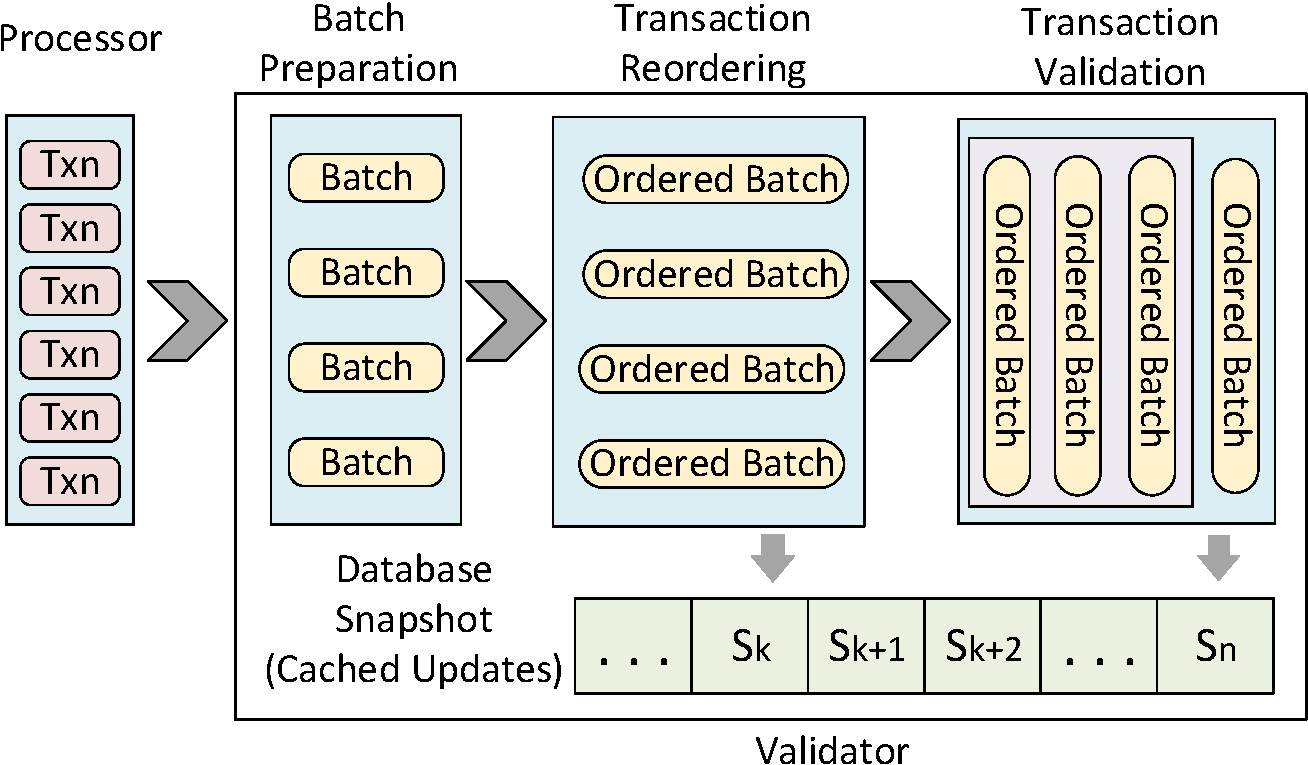
\includegraphics[width=1\columnwidth]{./figures/validator}
	\vspace{-2em}
	\caption{The architecture of parallel validator. It is decoupled into three subcomponents for pipeline parallelism: batch preparation, transaction reordering, and transaction validation. Each subcomponent can be further parallelized.}
	\vspace{-1em}
	\label{fig:reorder:validator}
\end{figure}
